\chapter{\textit{Wireless sensor networks} - WSNs}

Este capitulo aborda as principais técnicas de localização utilizando WSNs.

\label{wsn}
	WSNs é uma rede de sensores que coleta informações em um campo monitorado. Este tipo de rede tem sido utilizada em 
	várias aplicações, incluindo rastreamento de objetos, resgate, monitoramento de ambiente, entre outros \cite{omc}. Localização é um 
	tópico muito importante, pois, muitas aplicações das WSNs dependem do conhecimento das posições dos sensores. Na maioria das WSNs 
	os sensores são estáticos, mas a tendência em aplicações modernas é os sensores terem mobilidade.
	
	Há um conjunto de algoritmos de localização que utilizam WSNs. Onde o calculo da localização depende das informações 
	de localização dos nodos(que podem ser estáticos ou móveis) da rede. Esses algoritmos podem ser divididos em duas categorias: \textit{range-based}
	e \textit{range-free}. Algoritmos do tipo \textit{range-free} \cite{omc} \cite{wsnsLinear} geralmente requerem que os nodos conhecidos, estejam dentro 
	do raio de comunicação dos sensores em comum. Eles tem sido muito explorados pois não precisam de \textit{hardware} extra. Os algoritmos do tipo \textit{range-based},
	geralmente necessitam de algum tipo de \textit{hardware} especial, onde a posição de um certo nodo pode ser obtida a partir da posição ou direção dos nodos conhecidos por ele.
	
\section{TOA(\textit{Time of Arrival})}
	TOA é o tempo medido em que um sinal (rádio frequência, acústicos, ou outros) chega a um
receptor pela primeira vez depois de emitido\cite{gps}. O valor medido é o tempo de transmissão somado ao
atraso do tempo de propagação. Este atraso,$t_{i,j}$
, entre a transmissão do sensor i e recepção do sensor j, é igual a distância entre o transmissor e o receptor, 
$d_{i,j}$, dividido pela velocidade de propagação do sinal, $v_{p}$
. Esta velocidade para a rádio frequência é aproximadamente $10^{6}$  vezes mais rápida que a velocidade do som \cite{gps},
ou seja, 1 ms corresponde a 0,3 m na propagação sonora, enquanto para a rádio frequência, 1 ns corresponde a 0,3 m \cite{gps}.

O ponto chave das técnicas baseadas em tempo é capacidade do receptor de
estimar com precisão o tempo de chegada em sinais na linha da visão. Esta estimativa é prejudicada tanto pelo ruído 
aditivo quanto por sinais de multi percurso.

\section{TDOA(\textit{Time Difference of Arrival})}
  Os algoritmos de TDOA fazem a medição da diferença no tempo de recepção
de sinais de diferentes estações de base (Base Station's - BSs)), sem a necessidade de uma sincronização de
todos os participantes BSs e terminais móveis(MT)) \cite{tdoa}. Na verdade, a incerteza entre os tempos de referência
dos BSs e do MT pode ser removidas por meio de um cálculo diferencial. Por isso, apenas
os BSs envolvidos no processo de estimativa de localização deve ser bem sincronizados.

Para um par de BSs, digamos i e j, o TDOA,
$T_{ij}$, é dada por $T_{ij} TBSi - TBSj$, onde $TBSi$ e $TBSj$ são os tempos absolutos tomados 
pelo tempo de chegada nos BSs i e j, respectivamente. Supondo que o MT está em LOS (\textit{line-of-sight}) com ambos os BSs, i
e j, o MT deve situar-se em uma hipérbole. Uma segunda hipérbole, onde o
MT deve estar, pode ser obtido através de uma medição adicional de TDOA envolvendo
um terceiro BS. A posição do usuário pode ser identificada como o ponto de intersecção
das duas hipérboles. A solução do sistema de equações pode ser encontrado com um
método iterativo e minimização dos quadrados mínimos \cite{tdoa}.

O método dos quadrados mínimos procura encontrar 
o melhor ajuste para um conjunto de dados tentando minimizar a soma dos quadrados das diferenças 
entre o valor estimado e os dados observados (tais diferenças são chamadas resíduos).

Queremos estimar valores de determinada variável y. Para isso, consideramos os valores de outra variável x 
que acreditamos ter poder de explicação sobre y conforme a fórmula:

    y = $\alpha$ + $\beta$ x + $\varepsilon$

onde:
    \begin{itemize}
     \item $\alpha$: Parâmetro do modelo chamado de constante (porque não depende de x).
     \item  $\beta$: Parâmetro do modelo chamado de coeficiente da variável x.
     \item  $e$: Erro - representa a variação de y que não é explicada pelo modelo.
    \end{itemize}

Também temos uma base de dados com n valores observados de y e de x . 
O método dos mínimos quadrados ajuda a encontrar as estimativas de $\alpha$ e $\beta$.

O método dos mínimos quadrados minimiza a soma dos quadrado dos resíduos, ou seja, minimiza $\sum_{i=1}^n e_i^2$.

A ideia por trás dessa técnica é que, minimizando a soma do quadrado dos resíduos, encontraremos a e b que trarão 
a menor diferença entre a previsão de y e o y realmente observado.

\section{AOA(\textit{Angle of Arrival})}
A Localização baseada em AOA envolve a medição do ângulo de chegada de um sinal de uma BS
a um receptor ou vice-versa. Em qualquer um dos casos, uma única medida produz uma linha reta 
entre a BS e o receptor. A medida do ângulo de chegada com outra \textit{base station}
produzirá uma segunda linha reta e, a intersecção das duas linhas, vai fornecer a posição
do dispositivo\cite{aoa3}.
	\begin{figure}[hb]
	\centering
	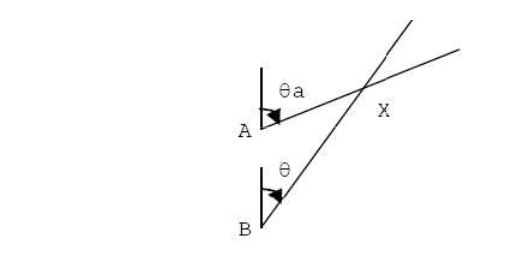
\includegraphics[scale=0.5]{images/aoa.png}
	\caption{Anglel of Arrival\cite{aoa3}. }
	\label{fig:aoa}
	\end{figure}
	
      Existem duas maneiras nas quais sensores medem o AOA \cite{aoa}. O método mais
comum é usar um vetor de sensores. Neste caso, cada nó sensor é
composto de dois ou mais sensores individuais (microfones para sinais acústicos ou antenas de sinais de rádio frequência),
cujas posições com relação ao centro do nó são conhecidos. A AOA é estimada a partir
das diferenças de tempos de chegada de uma transmissão do sinal em cada um dos elementos do vetor de sensores.

  A segunda abordagem para a estimativa do AOA, usa a razão RSS entre duas (ou
mais) antenas direcionais localizadas no sensor. Duas antenas direcionais apontadas em
direções diferentes, de tal maneira que suas hastes se sobrepõem, podem ser usadas para
estimar a AOA partir da relação entre seus valores individuais RSS.

\begin{comment}
AOA is defined as the angle between the propagation
direction of an incident wave and some reference direction,
which is known as orientation.
Orientation
, defined as a fixed
direction against which the AOAs are measured, is represent
ed
in degrees in a clockwise direction from the North. When
the orientation is 0
◦
or pointing to the North, the AOA is
absolute, otherwise, relative. One common approach to obta
in
AOA measurements is to use an antenna array on each sensor
node.We assume that the beacons have
no information about their orientations and the unknowns ca
n
detect the AOA information between neighbor nodes by using
one of the above methods

http://citeseerx.ist.psu.edu/viewdoc/download?doi=10.1.1.134.5991&rep=rep1&type=pdf
\end{comment}



\section{RSS(\textit{Received Signal Strength})}	
	A localização baseada em RSS apresenta-se como uma das únicas a não necessitar de \textit{hardware} extra, e ser uma técnica
de fácil aplicação. 
	
	Há três métodos de localização que utilizam a medição de RSS em WSNs: estação base mais forte, modelo de propagação e \textit{fingerprinting}.
	O primeiro método é o mais simples, a localização de um nodo da rede pode ser estimado como a posição do \textit{Access Points}(AP) mais próximo, no 
	qual o nodo se comunicou. Este método pode não atingir grande precisão devido a complexidade de WSNs em ambientes \textit{indoor} e 
	a limitação da cobertura do AP.
	
	No método de modelo de propagação, a medição do sinal no receptor e o valor
obtido indica a distância até o transmissor \cite{rss1}. Sem nenhuma interferência, a distância de dois nodos $i$ e $j$ pode ser 
relacionada com a força do sinal medido, através do modelo log-normal apresentado em \cite{rss2}:
\begin{comment}
In the wireless communication channel, the signal strength is related to the distance through the log-normal shadowing model [18]. 

Based on this model, the signal strength between the node Formula and the node Formula is given as follows; Based on this model, the signal strength between
the node i and the node j is given as follows
where
P0 is the path loss for the reference distance, and η is the path loss exponent, d(i,j) is the distance between node i and node j,
d0 is the reference distance, X σ is a Gaussian random variable of zero mean with standard deviation σ . If the obstructed interferencesdo not exist, the signal
strength rss(i,j) can be used directly for the localization procedure
	c
\end{comment}
	\begin{figure}[hb]
	\centering
	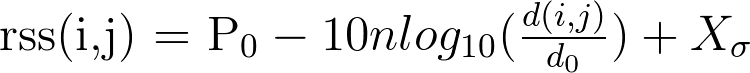
\includegraphics[scale=0.4]{images/CodeCogsEqn.png}
	\caption{Modelo Log-normal \cite{rss2}.}
	\label{fig:rssDist}
	\end{figure}
	
	Onde $P_0$ é a perda de percurso para a distância de referência,
$n$ á o expoente de perda de percurso, $d(i,j)$ é a distância entre os nodos $i$ e $j$,
$d_0$ é a distância de referencia, $X_\sigma$ é uma variável aleatória Gaussiana de média zero com desvio padrão $\sigma$.

Tal forma de medição por muitas vezes é
descartada, pois não leva em conta o ambiente onde está sendo aplicada a medição; logo,
corresponde a um resultado não confiável, obstruções e obstáculos proporcionam erros de grande relevância, 
sendo esse um dos maiores problemas dos métodos de localização baseados em RSS, várias técnicas foram propostas para 
contornar esse problema como pode ser visto em \cite{wifiRadar}\cite{rss1}\cite{wsnsLinear}\cite{multAgent} \cite{rss2}.

A figura abaixo mostra como a estimativa da real posição de um nodo é afetado pela interferências de obstrução:
	\begin{figure}[ht]
	\centering
	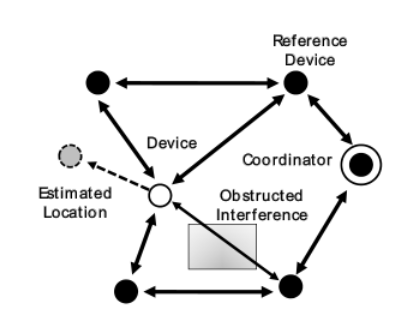
\includegraphics[scale=0.5]{images/rsserror.png}
	\caption{Influência de um obstáculos na localização de um nodo\cite{rss1}. }
	\label{fig:rsserror}
	\end{figure}
	
	Recentemente, localização em WSNs baseado em RSS \textit{fingerprinting} tem se tornado uma das técnicas mais exploradas 
	em ambientes \textit{indoor}\cite{fingerPrint}\cite{wifiRadar}\cite{fingerPrint2}. Comparada com as outras duas técnicas, \textit{fingerprinting} é facilmente empregada 
	e é tolerante ao ruido do sinal, e isso permite uma maior precisão em relação aos outros. Este método normalmente é composto por duas fases: 
	aprendizado e determinação. Na primeira fase o objetivo é construir uma tabela para cada coordenada de amostras de RSS 
	de alguns APs. Na fase de determinação, o nodo informa uma amostra do RSS que é comparada com cada entrada do tabela, o registro
	que mais se aproxima da amostra informada é adotada como atual posição do nodo.
	
   Em \cite{wifiRadar} - \textit{"Radar: an in-building RF-based user location and tracking system"}, Bahl e Padmanabhan propõem o método empírico,
   para localização baseada em RSS \textit{indoor}. O método consiste em realizar uma série de medições da força de sinal das estações bases, 
   e a partir dessas medições, a localização pode ser determinada fazendo uma triangulação dos dados coletados. 

  No artigo \cite{wifiRadar}, para obter a posição de um nodo, são medidas as forças do sinal wifi de três \textit{access points} (rss1, rss2, rss3), 
utiliza-se a distância Euclidiana, para fazer a comparação com os dados previamente coletados $sqrt((rss1-rss1')^{2}+(rss2-rss2')^{2}+(rss3-rss3')^{2})$, 
e assim encontrar o ponto que mais se aproxima dos parâmetros coletados naquele local. 
	
	A precisão da técnica de \textit{fingerprinting} reside nas amostras de RSS, qualquer mudança no ambiente como 
	reposição de APs, retirada ou inclusão de objetos e o trafego de pessoas no local podem interferir no desempenho desta técnica. 
	Esse é o principal problema dessa técnica.


